\subsection{Details of Hardware Simulation}
\label{emt:sec:details_hwsim}

\schaic{Shall we consider removing this section if we elaborated ECPT and FPT results in Sec 8?}
\noindent
Figure~\ref{emt:fig:hwsim} provides detailed results 
    of the hardware simulation 
    in \S\ref{emt:sec:eval:hwsim}.
We collect the instruction traces and memory traces by running the macro benchmarks
    and application workloads on EMT-Linux using our emulator,
    and use the traces for hardware simulation, as shown in Figure~\ref{emt:fig:eval:emulator}.
We use DynamoRIO~\cite{plat:dynamorio} as the hardware simulator
    to model the CPU described in the ECPT paper (Table 2 in~\cite{skarlatos2020ecpt}).
%    our emulator toolchain supports different backends such as Gem5 and SST.

% \begin{figure}[t]
% 	\centering
% \begin{subfigure}[b]{0.4\textwidth}
% 	\centering
% 	
\includegraphics[width=\textwidth]{data/ecpt_legend.pdf}
% 	\vspace{-0.6cm}
% \end{subfigure}
% \begin{subfigure}[b]{0.235\textwidth}
% 	\centering
% 	% 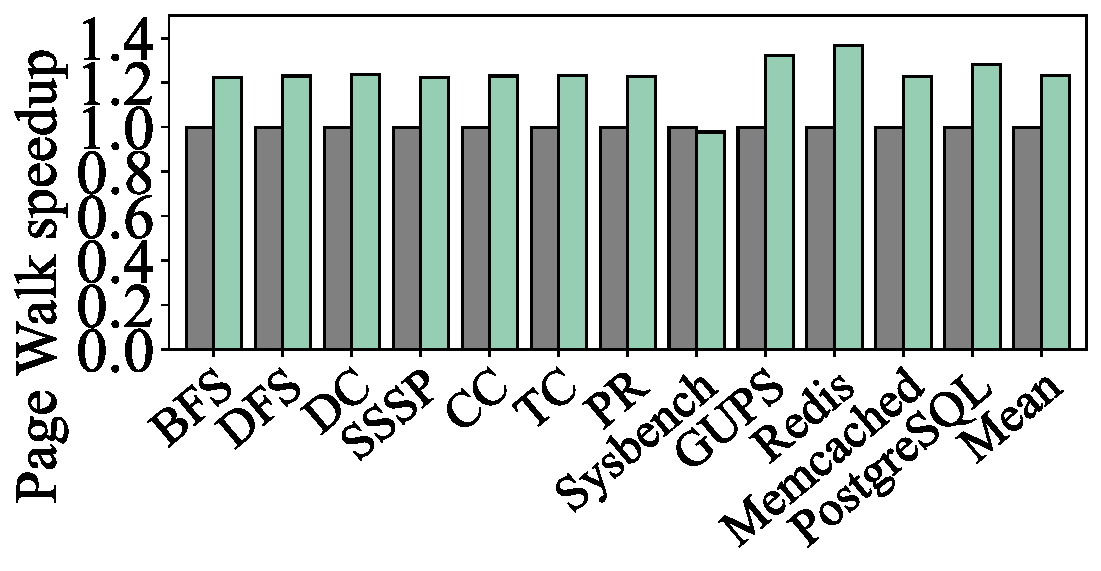
\includegraphics[width=\textwidth]{data/ecpt_pgwalk_unified_never.pdf}
% 	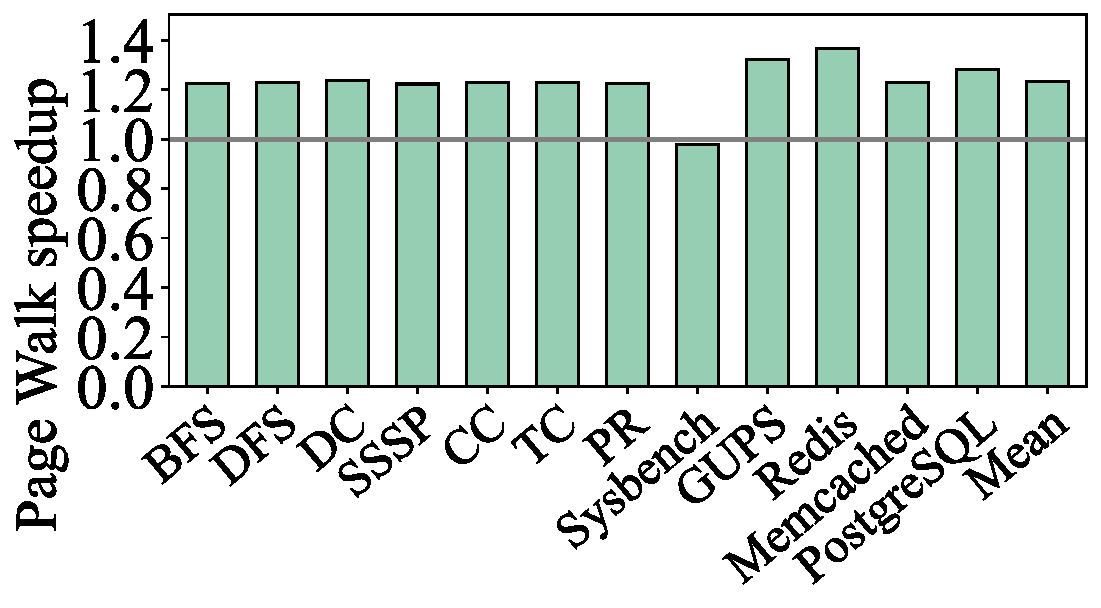
\includegraphics[width=\textwidth]{data/ecpt_pgwalk_unified_never_single.pdf}
% 	% \vspace{-0.1cm}
% 	\vspace{-20pt}
% 	\caption{Page table walk latency}
% 	\label{emt:fig:eval:eval:pw-4KB}
% 	\end{subfigure}%
% 	\begin{subfigure}[b]{0.235\textwidth}
% 	\centering
% 	% 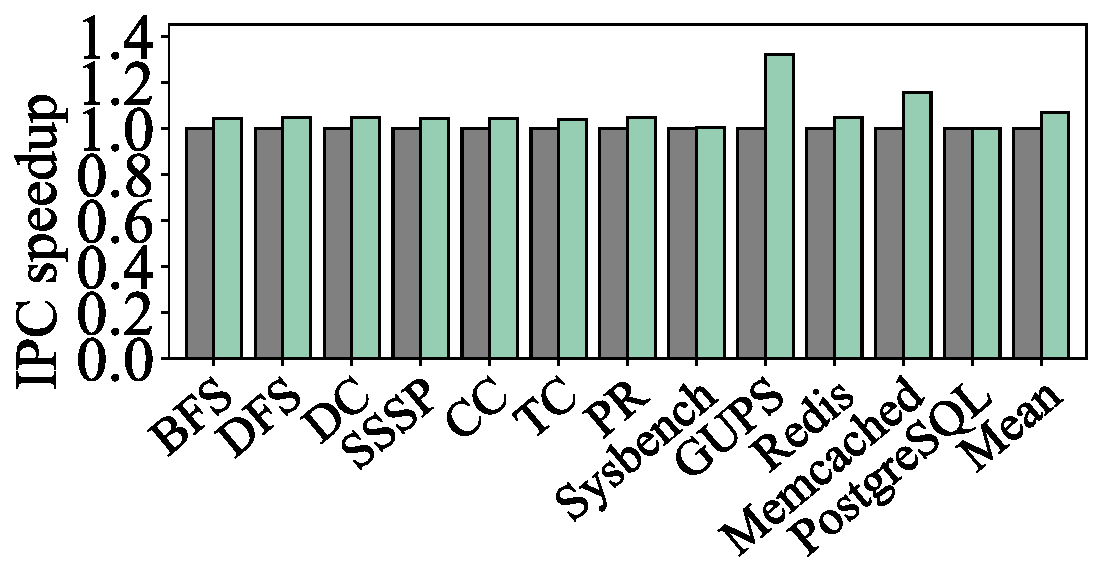
\includegraphics[width=\textwidth]{data/ecpt_ipc_unified_never.pdf}
% 	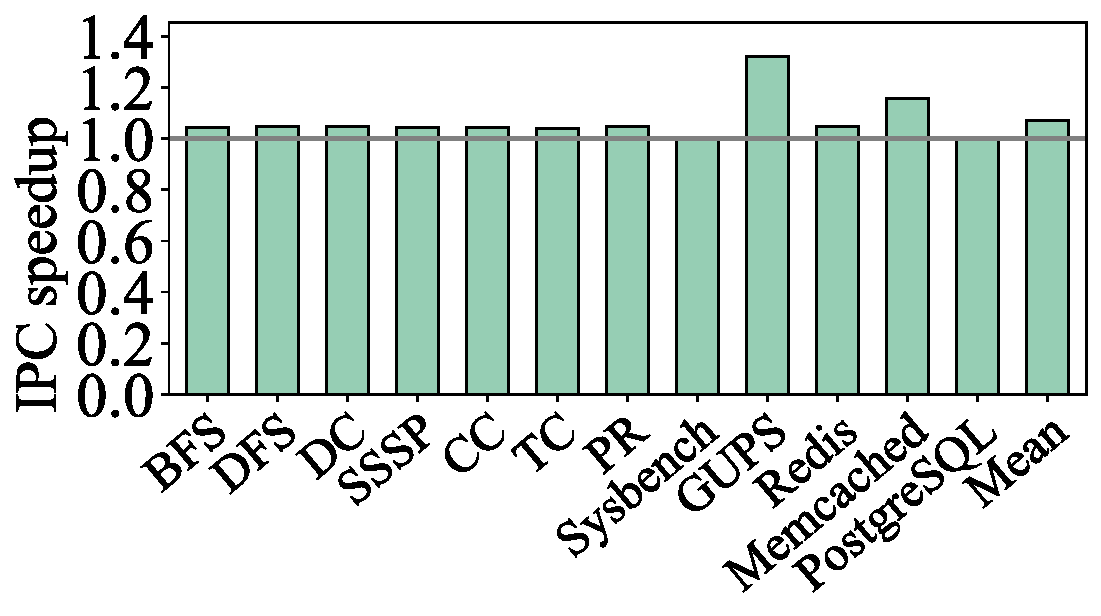
\includegraphics[width=\textwidth]{data/ecpt_ipc_unified_never_single.pdf}
% 	\vspace{-20pt}
% 	\caption{IPC}
% 	\label{emt:fig:eval:eval:ipc-4KB}
% 	\end{subfigure}
	
% \begin{subfigure}[b]{0.235\textwidth}
% 	\centering
% 	% 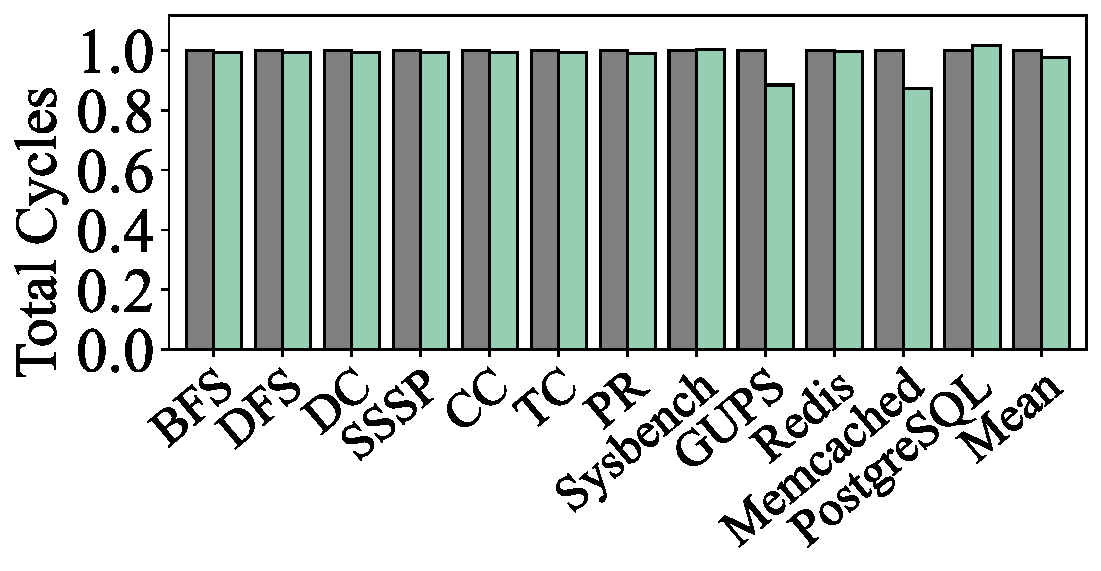
\includegraphics[width=\textwidth]{data/ecpt_e2e_unified_never.pdf}
% 	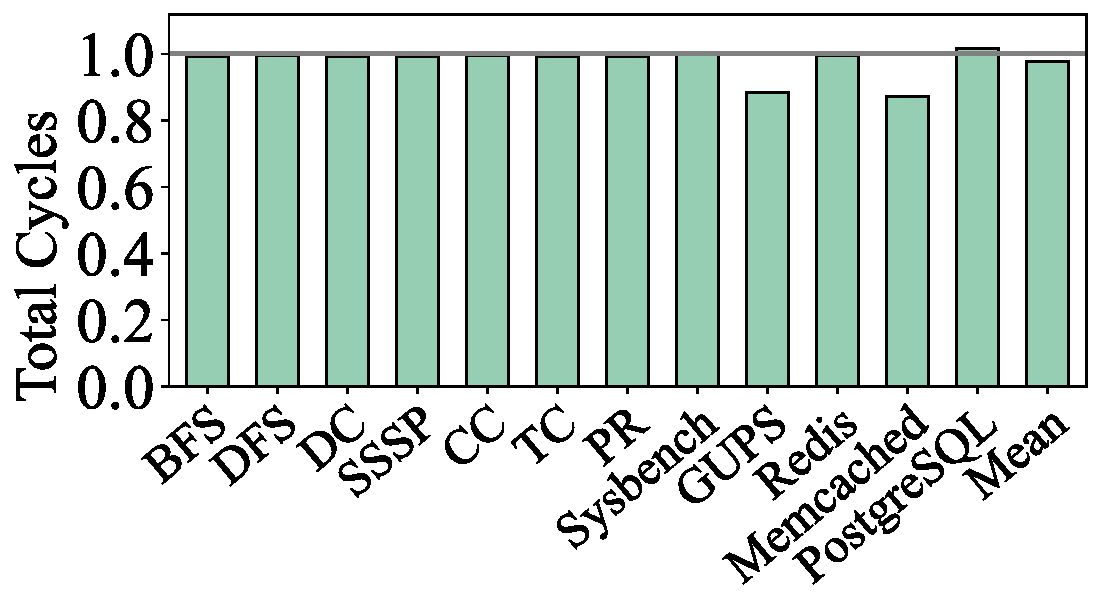
\includegraphics[width=\textwidth]{data/ecpt_e2e_unified_never_single.pdf}
% 	\vspace{-20pt}
% 	\caption{Total cycles}
% 	\label{emt:fig:eval:eval:e2e-4KB}	
% \end{subfigure}
% \begin{subfigure}[b]{0.235\textwidth}
% 	\centering
% 	% 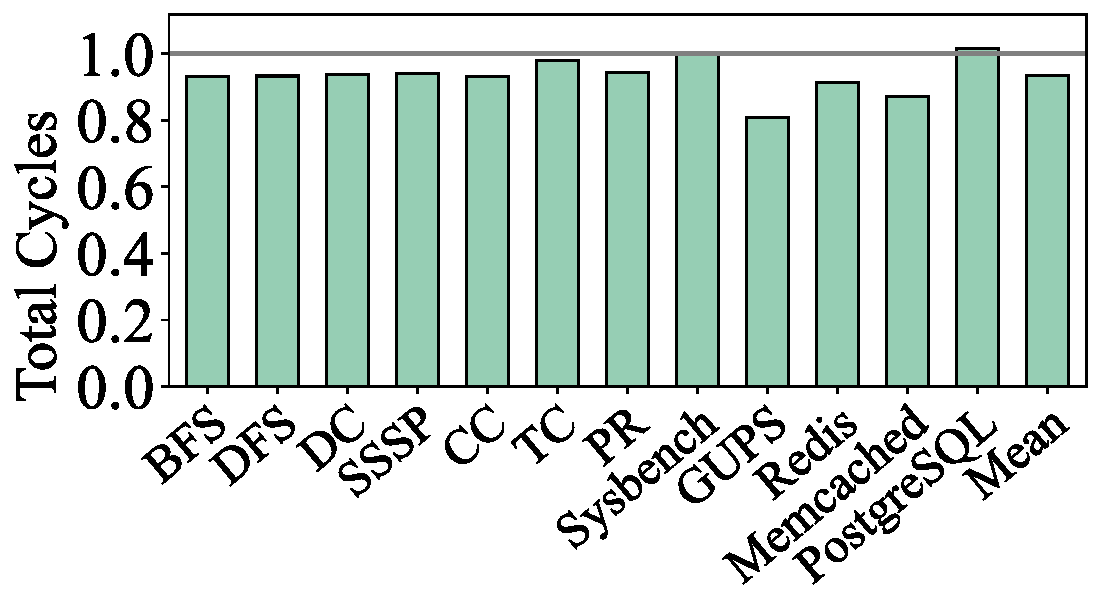
\includegraphics[width=\textwidth]{data/ecpt_e2e_running_never.pdf}
% 	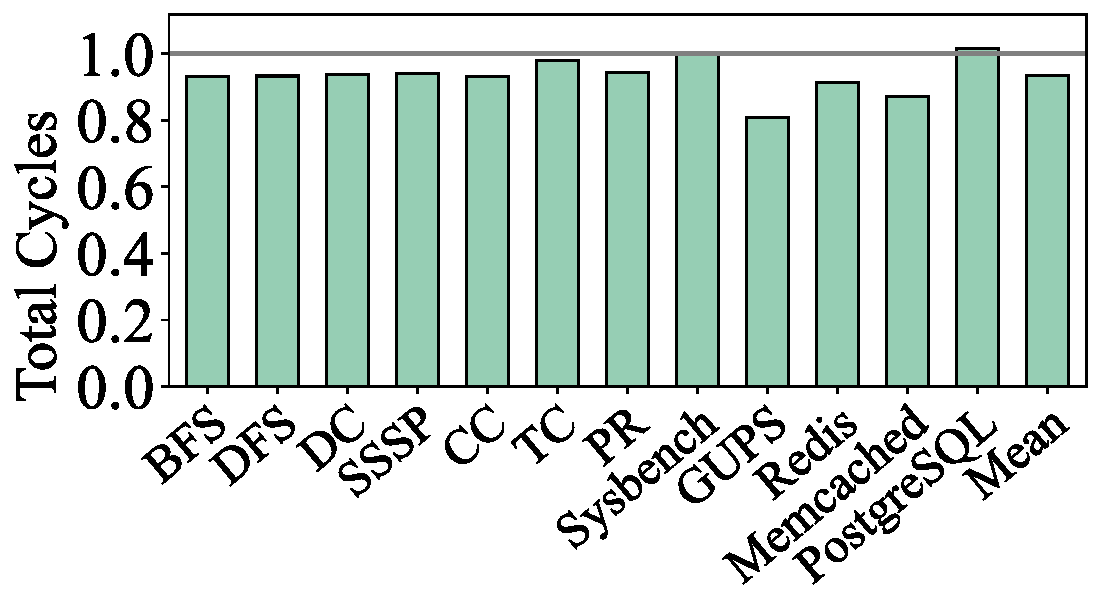
\includegraphics[width=\textwidth]{data/ecpt_e2e_running_never.pdf}
% 	\vspace{-20pt}
% 	\caption{Total cycles (running phase)}
% 	\label{emt:fig:eval:eval:e2ert-4KB}
% \end{subfigure}
% \vspace{-20pt}
% \caption{{\bf Simulation results in terms of Page Table Walk Latency, 
%     Instruction Per Cycle (IPC) and Total Cycles with the ECPT system 
%     and the x86-64 system, running EMT-Linux.} All results are normalized
%     to those of the x86-64 system as the baselines.}
% \label{emt:fig:hwsim}
% % \vspace{-5pt}
% \end{figure}

% EMT-Linux does not assume the execution platform,
%	so it can be run unmodified in the simulators commonly used in architectural research (e.g., gem5~\cite{plat:gem5}, DynamioRIO~\cite{plat:dynamorio}, SST~\cite{plat:sst}, or qemu~\cite{plat:qemu}).
% EMT can help researchers evaluate the software characteristics of their architectural designs,
%	providing them with new understandings and insights,
%	without disrupting the hardware performance results.

% We measure page walk latency,  (IPC), and total cycles across the macro benchmarks 
%	and real world applications
%	running on the \eradix and \eecpt. The methodology of such evaluation is discussed in .
\subsubsection{Traditional Hardware Metrics}

\noindent
Figure~\ref{emt:fig:eval:eval:pw-4KB} and \ref{emt:fig:eval:eval:ipc-4KB}
	shows the speedup of ECPT over x86-64 Radix in terms of 
    Page Table Walk Latency and Instructions Per Cycles (IPC).
These two metrics are considered key performance metrics of hardware translation schemes~\cite{skarlatos2020ecpt,park2022fpt}
    and are widely used in hardware architecture research.
Based on these two metrics, ECPT has significant performance advantages over x86-64 Radix.
Specifically, on average, ECPT speeds up page table walks by 23.1\%
	and increases IPC by 7.0\%.
For most workloads, ECPT directly fetches the translation entries using its hashing-based translation,
    avoiding the overhead of walking the x86-64 page table tree.
%	instead of walking the  accessing intermediate page tables as radix does.
The only exception is Sysbench whose workload has a very high Page Walk Cache (PWC) hit rate of 99.8\%
    at the PMD level on x86-64, i.e., 
	the page table walks skip almost all the intermediate steps and directly accesses last-level PTEs.
Meanwhile, ECPT pays extra cycles for hash computation in addition to CWC accesses,
    so it has a slightly slower page table walk and IPC.
Overall, ECPT is very effective in reducing page table walk latency and improving IPC.

The results show the same trends as the ECPT paper~\cite{skarlatos2020ecpt},
    but the concrete numbers differ due to different simulation infrastructures
    and the MMU implemenations in the simulators.
The original ECPT paper uses the proprietary Simics simulator as the frontend with a modified
    SST simulator as the backend, while the EMT toolchain uses open-source QEMU as the frontend 
    and DynamioRIO as the backend.
We were not able to acquire the Simics-based simulator, which is also a motivation 
    for us to build an open-source toolchain as an open platform for 
    hardware-software research.

\subsubsection{Metrics with OS Overhead Considered}

\noindent
Although IPC is often used as a metric of application performance,
    it only measures instruction throughput but does not reflect application runtime.
For the ECPT system, despite that
	ECPT increases IPC, 
    our ECPT MMU driver introduces more kernel instructions than the x86-64 MMU driver (\S\ref{emt:ss:eval:eval-ecpt-os}).
Therefore, we include kernel overhead (mostly page fault handling as shown in Figure~\ref{emt:fig:eval:eval-kern-inst-breakdown}) 
	and measure the total cycles for running 
	macro benchmarks and applications.
The result is shown in Figure~\ref{emt:fig:eval:eval:e2e-4KB}.
Overall, the ECPT system reduces total cycles by 2.3\% on average.
GUPS and Memcached show major improvements, where the ECPT system reduces the total cycles 
	by 11.5\% and 12.9\%, because these two workloads involve low kernel work.


Note that all the evaluated macro benchmarks and application workloads have two 
    phases at runtime:
a {\it loading phase} to load data from the disk to memory,
and a {\it running phase} that runs the computation or serves user requests.
% We do not differentiate these fine-grained phases in our evaluation.
The running phase often has much lower kernel activities compared with the 
    loading phase.
If we only consider the running phase, then the ECPT system 
    reduces total cycles by 6.6\% on average compared to the 
    x86-64 system, as shown in Figure~\ref{emt:fig:eval:eval:e2ert-4KB}.

Through the aforementioned analysis, we show that the OS can play 
    an important role in application performance,
    which can be overlooked with hardware metrics.
\schai{Without building the OS memory management, it is hard to assess OS overhead accurately. 
Prior work assumed that OS overhead is constant under different memory-translation architectures. 
In the initial modeling, the memory trace is collected from running benchmarks on vanilla Linux on x86-64; 
	the trace is then replayed in a simulator of ECPT MMU. 
As shown in \S\ref{emt:ss:perf-ecpt}, memory translation architectures can have profound implications for OS performance. 
For example, in ECPT and other hashing-based translation schemes, range operations are inherently more expensive.} 
EMT aims to enable OS experience for new translation architectures.
\schai{We believe that EMT effectively lowers the barrier to implement OS support for new memory-translation architectures
by making the kernel developers focus on MMU driver implementation.
}
\schaic{This modifications originated from reviewrC's comments on comparison with the original ECPT paper.}

% Hence, initial modeling is inaccurate with regard to the OS performance/overhead. 
% Note: the OS implementation reveals design issues of the original ECPT scheme and evolves its architectural design.}

% \schai{Fundamentally, without building the OS memory management, it is hard to assess OS overhead accurately. 
% Prior work often assumes that OS overhead is constant under different memory-translation architectures. 
% In the initial modeling, the memory trace is collected from running benchmarks on x86-64 Linux; 
% 	the trace is then replayed in a simulator of ECPT MMU. 
% As shown in the paper, memory-translation architectures can have profound implications for OS overhead. 
% For example, in ECPT and other hashing-based translation schemes, range operations are inherently more expensive. 
% Hence, initial modeling is inaccurate with regard to the OS performance/overhead. 
% Note: the OS implementation reveals design issues of the original ECPT scheme and evolves its architectural design.}


% The original ECPT paper~\cite{skarlatos2020ecpt} doesn't reveal this signal since it focuses speedup analysis of user space instructions
%	and lack the tool to carry out the kernel performance analysis.
% The original ECPT paper also focuses on the stable stage of benchmarks which 
%	contains less than 1\% of kernel instructions.
%We also measure the cycles required during the application stable stage,
%	the results are in Figure~\ref{emt:fig:eval:eval:e2ert-4KB}.
% On average, EMT reduces the cycle count by 6.6\% for the stable stage.



    % 4KB
	% baseline        1.000000
	% + VMA opt       0.318733
	% + iterator opt  0.316050
	
	% THP
	% baseline        1.000000
	% + VMA opt       0.932852
	% + iterator opt  0.466743
	
% We can see that different optimizations lead to different benefits
% 	under different setups.
% Under a 4KB setup, the iterator optimization has little benefit 
% 	because the huge page optimization avoids the most expensive scanning
% 	of memory areas.
% On the other hand, with THP enabled, the huge page optimization does 
% 	not save much while the iterator leads to major benefits.

\begin{figure}
\centering
% % return addr_range_void(tentry, va, size) &&
\begin{subfigure}[b]{.5\textwidth}
\begin{minted}[xleftmargin=17.5pt,linenos,mathescape,breaklines,fontsize=\scriptsize,escapeinside=@@]{C}
bool thp_eligible(tobj, pg_size, vma) {
  if (pg_size == PMD_SIZE) 
    return pmd_none(*tobj->pmd) &&
      __transparent_hugepage_enabled(vma);
  ... // other page sizes
} /* arch/x86/mm/radix.c */
\end{minted}
\captionsetup{justification=centering}
\vspace{-10pt}
\caption{x86-64 MMU driver}
\end{subfigure}
\begin{subfigure}[b]{.5\textwidth}
\begin{minted}[xleftmargin=17.5pt,linenos,mathescape,breaklines,fontsize=\scriptsize]{C}
bool thp_eligible(tobj, pg_size, vma) {
  if (pg_size == PMD_SIZE){ 
    return __transparent_hugepage_enabled(vma) &&
      addr_range_void(tobj, 
        tobj->va & PMD_MASK, // start of 2MB range
        (tobj->va + PMD_SIZE) & PMD_MASK); // end of 2MB range
  }
  ... // other page sizes
} /* arch/x86/mm/ecpt.c */
\end{minted}
\captionsetup{justification=centering}
\vspace{-10pt}
\caption{ECPT MMU driver}
\label{emt:code:thpgen:ecpt}
\end{subfigure}
\vspace{-20pt}
\caption{\bf Different implementaions of the EMT customized function,
    \texttt{\small  thp\_eligible()}.}
\label{emt:code:thpgen}
\end{figure}

\subsection{More Hardware-Specific Optimizations}
\label{emt:sec:app:another}

\noindent
We discussed optimizations that are implemented using the 
    iterator customizable functions,
    both in the x86-64 MMU driver (Figure~\ref{emt:code:iternext})
    and in the ECPT MMU driver (\S\ref{emt:ss:ecpt-mmu-driver}).
In this section, we present another optimization through the customizable function,
    \texttt{\small thp\_eligible} in the huge page group.
The function checks if a huge page can be created in a Virtual Memory Area (VMA).
It is on the critical path of page fault handling for determining huge page faults,
    and is important.
% Its performance is important.

Figure~\ref{emt:code:thpgen} shows the implementaions of \texttt{\small thp\_eligible}
    in the x86-64 MMU driver and the ECPT MMU driver, respectively.
The two MMU drivers customize the default implemenation differently,
    due to different performance characteristics of the translation architectures.
The function returns the result of the AND operation of two condition checks:
1) if the virtual address range of the huge page contains any 4KB page mappings, 
and
2) if the VMA allows a huge page to be created (based on the VMA's attributes like size and alignment).
It is important to place the cheaper check first.
For x86-64 radix-tree page table, the first check is a cheaper check, 
    as it involves a single PMD entry lookup.
In contrast, ECPT has more expensive range operations like \texttt{\small addr\_range\_void()}
    (see the discussion in \S\ref{emt:sec:ecpt:os:perf});
    therefore, the order of the checks is opposite to that in 
    the x86-64 MMU driver.

%      baseline  iterator only  hugepage only  iterator + hugepage
% 4KB       1.0       0.451086       0.318733             0.316050
% THP       1.0       0.483435       0.932852             0.46674
Figure~\ref{emt:fig:eval:appendix} shows the effectiveness of this performance 
    optimization in the ECPT system,
    together with the iterator optimization 
    (which is discussed in Figure~\ref{emt:fig:eval:eval-ecpt-flame-thp}).
% ~\ref{emt:fig:eval:eval:opt-group-effect-4k} and~\ref{emt:fig:eval:eval:opt-group-effect-thp}
%	compare the effect of the iterator
%	optimization with the huge page optimization (\texttt{thp\_eligible}) in Figure~\ref{emt:fig:api-cus}.
We measure the number of instructions executed in the page fault handler
	when running GraphBIG BFS.
The \texttt{\small thp\_eligible} optimization is particularly effective in the 4KB setup,
    which reduces the number of instructions to 31.9\% of the baseline.
With the \texttt{\small thp\_eligible} optimization in place, 
    the iterator optimizations have little
    benefits, because most expensive memory scanning has already been avoided.
On the other hand, when THP is enabled, the check is true for most VMA,
	so page fault handler cannot skip expensive memory scanning in ECPT.
Hence, the \texttt{\small thp\_eligible} optimization does not save 
    much, while the iterator leads to significant benefits.

\begin{figure}
	\centering
	\begin{subfigure}[b]{0.4\textwidth}
		\centering
		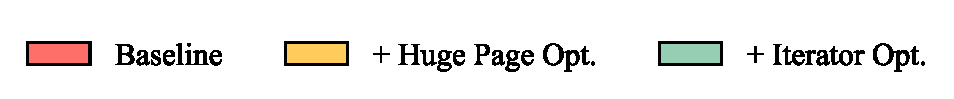
\includegraphics[width=\textwidth]{data/opt_group_effect_always.legend.pdf}
		\vspace{-0.6cm}
	\end{subfigure}
	\vskip\baselineskip
\begin{subfigure}[b]{0.24\textwidth}
	\centering
	\vspace{-10pt}
	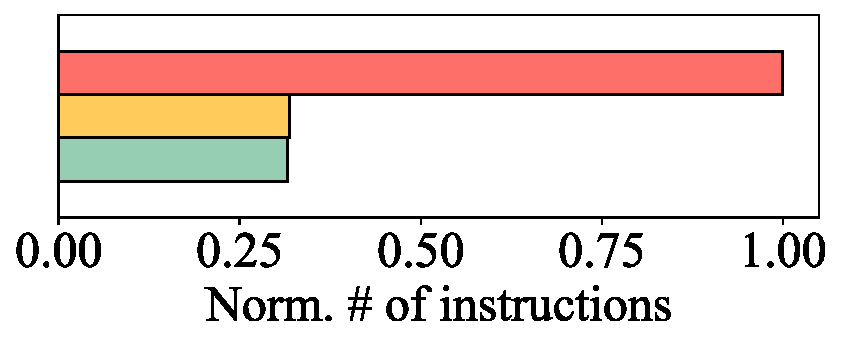
\includegraphics[width=\textwidth]{data/opt_group_effect_never.pdf}
	% \vspace{-0.1cm}
	\vspace{-18pt}
	\caption{4KB}
	\label{emt:fig:eval:eval:opt-group-effect-4k}
\end{subfigure}%
	% Subfigure 2
	% \vspace{-2cm}
	% \vspace{0.1cm}
	% \vspace{pt}
\begin{subfigure}[b]{0.24\textwidth}
	\centering
	\vspace{-10pt}
	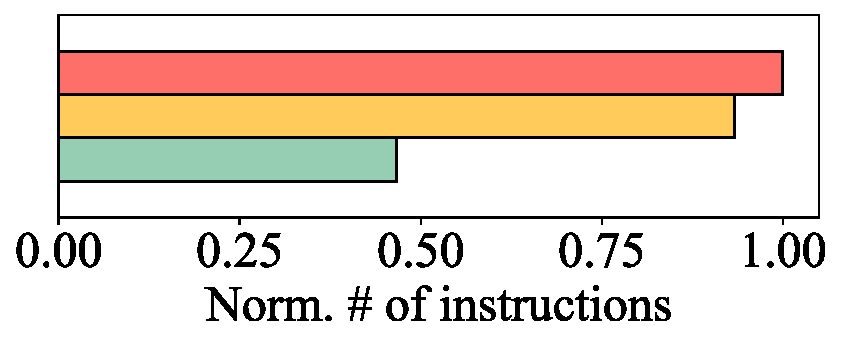
\includegraphics[width=\textwidth]{data/opt_group_effect_always.pdf}
	% \vspace{-0.1cm}
	\vspace{-18pt}
	\caption{THP}
	\label{emt:fig:eval:eval:opt-group-effect-thp}
\end{subfigure}
	\vspace{-20pt}
	\caption{\bf Effectiveness of the iterator optimization and the \texttt{\small thp\_eligible}
        optimization on page fault handling 
		running GraphBIG BFS on the ECPT system.}
    \label{emt:fig:eval:appendix}
	% \schaic{If we really need space, we can make EMT-radix as a line.}
\end{figure}

\begin{comment}


We further use flame graphs~\cite{tool:flamegraph} to visualize
	fine-grained profiling data. A flame graph shows the stack frames of a
	program. We capture and report only the interesting functions. The
	length of the bars represents the number of instructions executed by each function.
Figures~\ref{emt:fig:eval:eval-radix-never-vs-ecpt-never-flame-a} and~\ref{emt:fig:eval:eval-radix-never-vs-ecpt-never-flame-b} 
	show the kernel instructions running GraphBIG
	BFS on EMT-Linux with the Radix
	and ECPT MMU drivers, respectively.
% Radix total inst: 112,288,315
% Radix PF handler: 85,381,622
% ECPT total inst: 175,012,292
% ECPT PF handler: 147,646,869
% ECPT leads to 1.56x more kernel work,
% 	in terms of the number of instructions,
% 	than with the Radix MMU driver.
% Specifically, for page fault handling,
% 	ECPT takes	
% 	1.73x more work than Radix.
% unified approach: beginning of loading + running stage
% Radix total inst: 116255504.6
% Radix PF handler: 84870978.55
% ECPT total inst: 178644432.7
% ECPT PF handler: 146765968.6
ECPT leads to 1.54x more kernel work,
	in terms of the number of instructions,
	than with the Radix MMU driver.
Specifically, for page fault handling,
	ECPT takes	
	1.73x more work than Radix.



% \schaic{The plot ~\ref{emt:figure:eval:eval-kern-inst-breakdown} above needs to be modified in format, recapture loading phase data, as well as add gups and sysbench data}.
% \schaic{In loading phase, the timer effect will not be significant, so I feel acceptable to include timer. 
% However, in later phase, we exclude timer, I will remove it for now.}

With ECPT,
	the EMT interface triggered 38.42\% of the kernel work (orange color);
	38.25\% of the instructions were spent on 
	page table insertion and lookup (blue color).
In contrast, EMT-Linux with Radix only spends 
	3.55\% of its kernel work in page-table-related operations.
% The difference in page table operation overheads account for xxx\% of 
% 	the total kernel work difference between \eradix and \eecpt shown in xxx (Previous figre, to be added).
The difference comes from the ECPT design that needs to
	compute hashes, resolve collisions (for insertion), 
	and search entries in multiple locations (for lookup).
Unlike hardware MMUs, it is hard for OS software to do parallel lookups
	on ECPT ways
	(which would involve task scheduling with high overhead).

\begin{figure}
\centering
\begin{subfigure}[b]{0.35\textwidth}
	\centering
	
\includegraphics[width=\textwidth]{data/flame_legend.pdf}
	\vspace{-0.6cm}
\end{subfigure}
\vskip\baselineskip
\vspace{-5pt}
\begin{subfigure}[b]{0.49\textwidth}
	\centering
	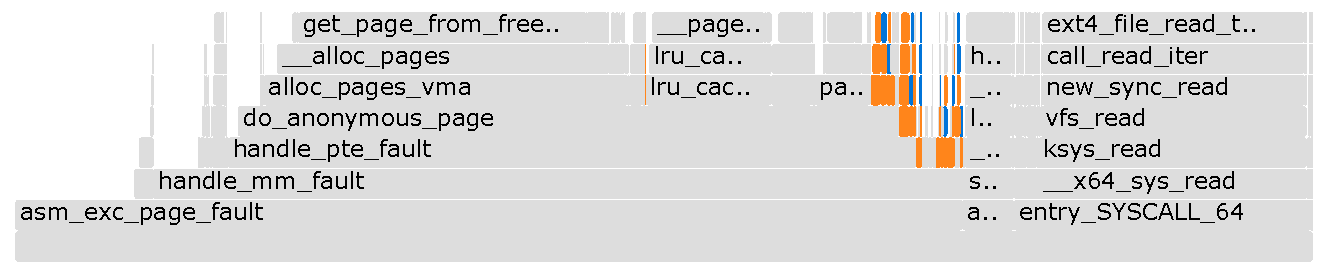
\includegraphics[width=\textwidth]{data/radix_never_graphbig_bfs_kern_inst.pdf.corrected.pdf}
	% \vspace{-0.1cm}
	\vspace{-15pt}
	\caption{Radix MMU driver}
	\label{emt:fig:eval:eval-radix-never-vs-ecpt-never-flame-a}
\end{subfigure}%
	\newline % This starts a new line
	% Subfigure 2
	% \vspace{-2cm}
	% \vspace{0.1cm}
	% \vspace{pt}
	\vspace{-20pt}
\begin{subfigure}[b]{0.49\textwidth}
	\centering
	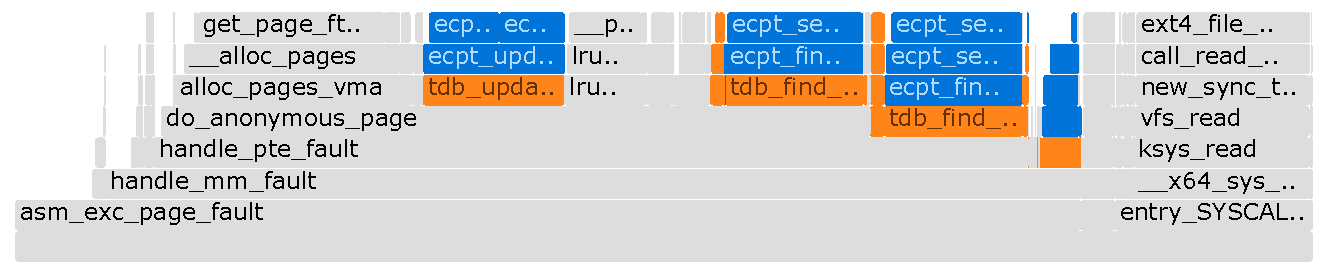
\includegraphics[width=\textwidth]{data/ecpt_never_graphbig_bfs_default_kern_inst.pdf.corrected.pdf}
	\vspace{-15pt}
	\caption{ECPT MMU driver}
	\label{emt:fig:eval:eval-radix-never-vs-ecpt-never-flame-b}
\end{subfigure}
	\vspace{-20pt}
	\caption{\bf Flame graph of EMT-Linux kernel instructions when running GraphBig BFS (no THP).}
	\vspace{-10pt}
\end{figure}
\end{comment}